\chapter{Resolving some ad hoc decisions from de Boer (2000)}
\label{ch:improving_de_boer}

In the previous chapter, we discussed the re-implementation of the imitation games as proposed by \citet{deBoer2000}.
We mentioned that both the vocal synthesizer and bark conversion were interpolated from publicly available data.
The calculations for determining effective second formant weight ($F'_2$) were found rather ad hoc and definitions varied between the paper and the available code.

We think the design decision to model the vocal tract from interpolated data is understandable in this context.
Not only is it faster than modelling a more complex synthesizer, but the fact that 18 different vowels were used for the interpolation makes it a reasonable approximation.
Especially when considering far fewer sounds were learned on average by the agents due to the limited acoustic space, we think the interpolated vocal tract doesn't impose a conflict for the study.
However, the interpolated bark conversion and calculations for $F'_2$ were something we think could influence the results.
For this reason, this chapter will go into detail on how we tested variants for these calculations using the alternative bark operator.

%------------------------------------

\section{Alternative bark conversion}
\label{sec:alternative_bark_conversion}

When discussing the \texttt{Bark Operator} class in section \ref{sec:reimplementing_perceive} we mentioned the inclusion of the optional \texttt{alternative\_bark\_conversion} parameter.
When this parameter is set to \texttt{True} both the conversion from Hertz to bark and back as well as the $F'_2$ calculations will differ from those described in Equation \ref{eq:bark_conversion_de_boer} and \ref{eq:f2_conversion_de_boer} respectively.

It was found that there is no single definition for the bark scale.
After comparing multiple variants we decided to settle for the bark conversion used by MatLab\footnote{\url{https://nl.mathworks.com/help/audio/ref/hz2bark.html}}.
The conversion from Hertz to bark is given in Equation \ref{eq:bark_conversion_matlab}.
The inverse can analytically be derived and was tested in the \texttt{2\_recreating\_de\_boer\_2000.ipynb} notebook.

\begin{equation}
\begin{aligned}
  \texttt{intermediate} &= \frac{26.81 * Hz}{1960 + Hz} - 0.53 \\
  bark &= 
    \begin{cases}
      \texttt{intermediate}+(0.15 * (2-\texttt{intermediate})) & \text{if } bark < 2 \\
      \texttt{intermediate}+(0.22 * (\texttt{intermediate} - 20.1)) & \text{if } bark > 20.1 \\
      \texttt{intermediate} & \text{else}
    \end{cases} 
\end{aligned}
\label{eq:bark_conversion_matlab}      
\end{equation}

%------------------------------------

\section{Alternative effective second formant calculation}
\label{sec:alternative_second_formant}

For the calculation of the effective second formant weight ($F'_2$), \citet{deBoer2000} stated that the strategy used by \citet{Schwartz1997} would probably be better.
For that exact reason, we implemented the strategy proposed by \citet{Schwartz1997}.
This strategy consists of two parts, determining a value $c$ and calculating $F'_2$ based on that $c$.
The process to determine $c$ is described in Figure \ref{fig:effective_second_formant}.
After $c$ is determined, $F'_2$ can be calculated.
This is done by using Equation \ref{eq:effective_second_formant}.
It is noted that \citet{Schwartz1997} used yet another bark conversion method.

\begin{figure}[H]
    \centering
    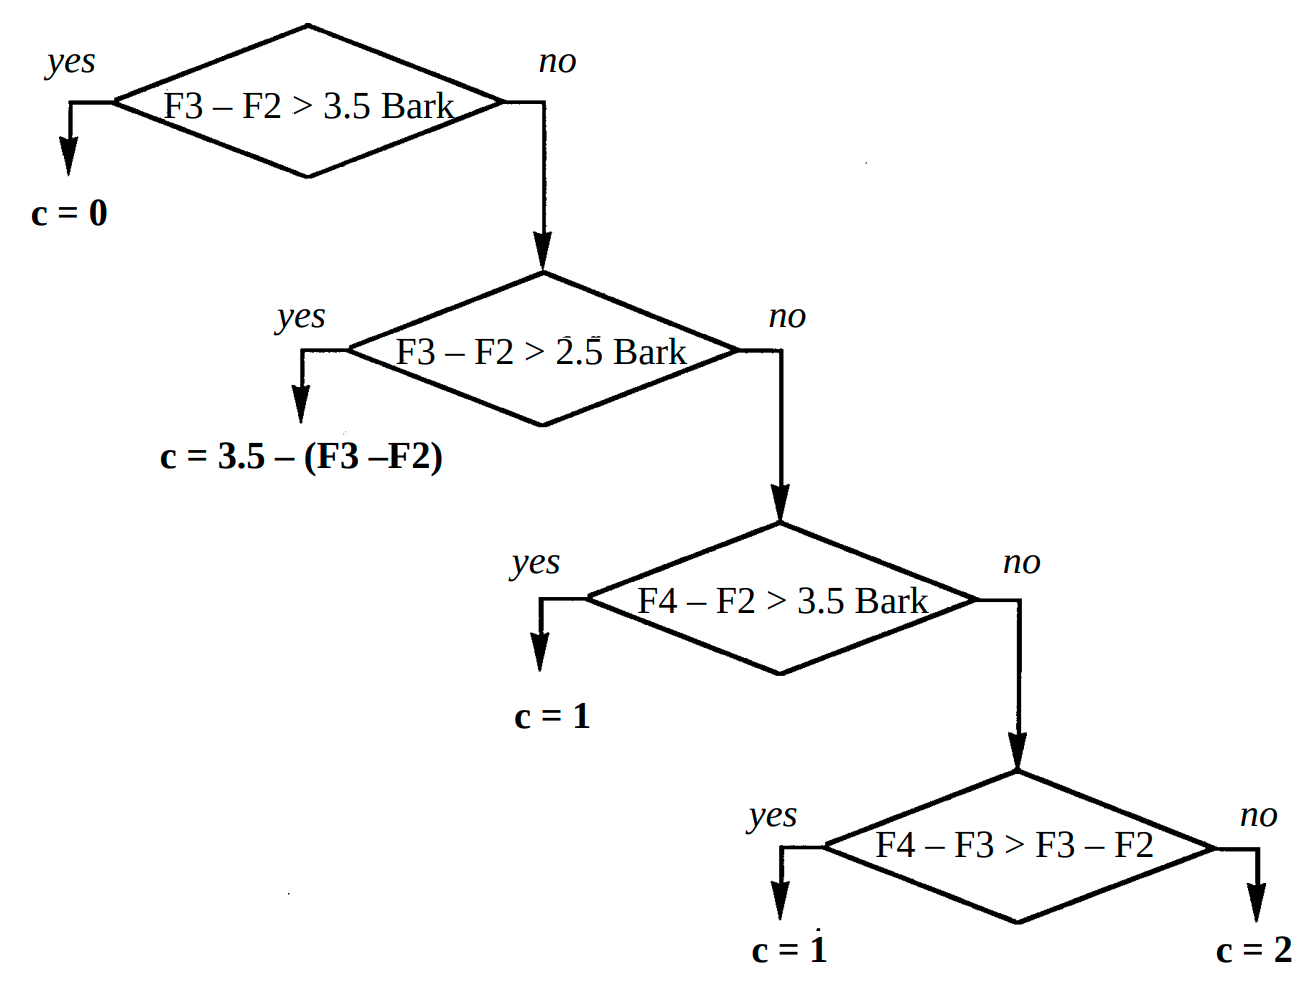
\includegraphics[width=0.5\linewidth]{images/improving/effective_second_formant.png}
    \captionsetup{width=\linewidth}
    \captionsetup{justification=centering}
    \caption{C calculation for effective second formant equation. Strategy and figure by \citet{Schwartz1997}}.
    \label{fig:effective_second_formant}
\end{figure}

\begin{equation}
  F'_2 = \frac{c_2F_2 + c_3F_3 + c_4F_4}{c_2 + c_3 + c_4}
    \begin{cases}
      c_2 = 1, c_3 = 0, c_4 = 0 & \text{if } c = 0 \\
      c_2 = 1, c_3 = 0.5, c_4 = 0 & \text{if } 0 \leq c \leq 1 \\
      c_2 = 0, c_3 = 1, c_4 = 0.5 & \text{else}
    \end{cases} 
\label{eq:effective_second_formant}      
\end{equation}

%------------------------------------

\section{Reachable acoustic space}
\label{sec:reachable_acoustic_space}

To visualise the impact of the change \texttt{Bark Operator} the reachable acoustic space was approximated by plotting multiple points.
This experiment is visualised in Figure \ref{fig:acoustic_reach}.
The alternative implementation visually differs in multiple ways.
As computer scientists, we find the more continuous nature of the implementation by \citet{deBoer2000} more pleasing.
However, an expert should ideally determine which of the two is more realistic.
In Chapter \ref{ch:results} it is discussed that the results of the experiment remain similar independent of the used variant.

\begin{figure*}[ht]
    \centering
    \begin{subfigure}{.45\textwidth}
        \centering
        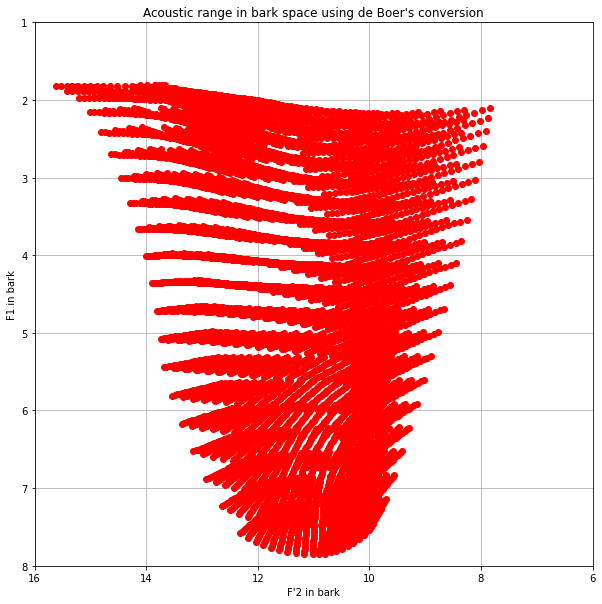
\includegraphics[width=\textwidth]{images/improving/reachable_acoustic_space-de_boer.png}
        \captionsetup{width=0.9\linewidth}
        \captionsetup{justification=centering}
        \caption{Default implementation}
    \end{subfigure}
    \hspace{0.5cm}
    \begin{subfigure}{.45\textwidth}
        \centering
        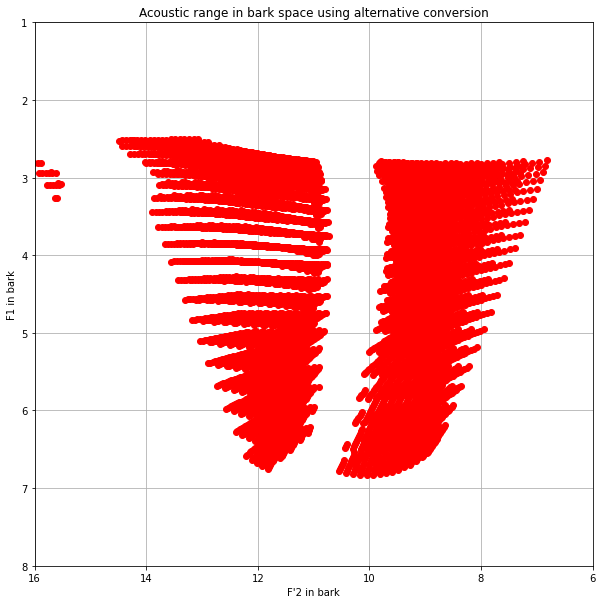
\includegraphics[width=\textwidth]{images/improving/reachable_acoustic_space-alternative.png}
        \captionsetup{width=0.9\linewidth}
        \captionsetup{justification=centering}
        \caption{Alternative implementation}
    \end{subfigure}
    \captionsetup{width=0.8\linewidth}
    \captionsetup{justification=centering}
    \caption{Reachable acoustic space of both Bark Operator alternatives.}
    \label{fig:acoustic_reach}
\end{figure*}